\section{\texttt{ex040.MF\_choke.xlsm} - Расчет штуцера}

Для контроля дебита и/или давления на добывающих скважинах вблизи устья может устанавливаться штуцер. Для штуцера, как для любого гидравлического элемента, возможно 4 варианта расчета - расчет давления по потоку, расчет давления против потока, расчет потока по давлениям и настройка модели штуцера по известным давлениям и потоку. В упражнении демонстрируются все варианты расчета. 

Файл примера \mintinline{vb.net}{ex040.MF_choke.xlsx} можно найти в папке \texttt{exercises} репозитория \unf{}.

\begin{figure}[h!]
	\center{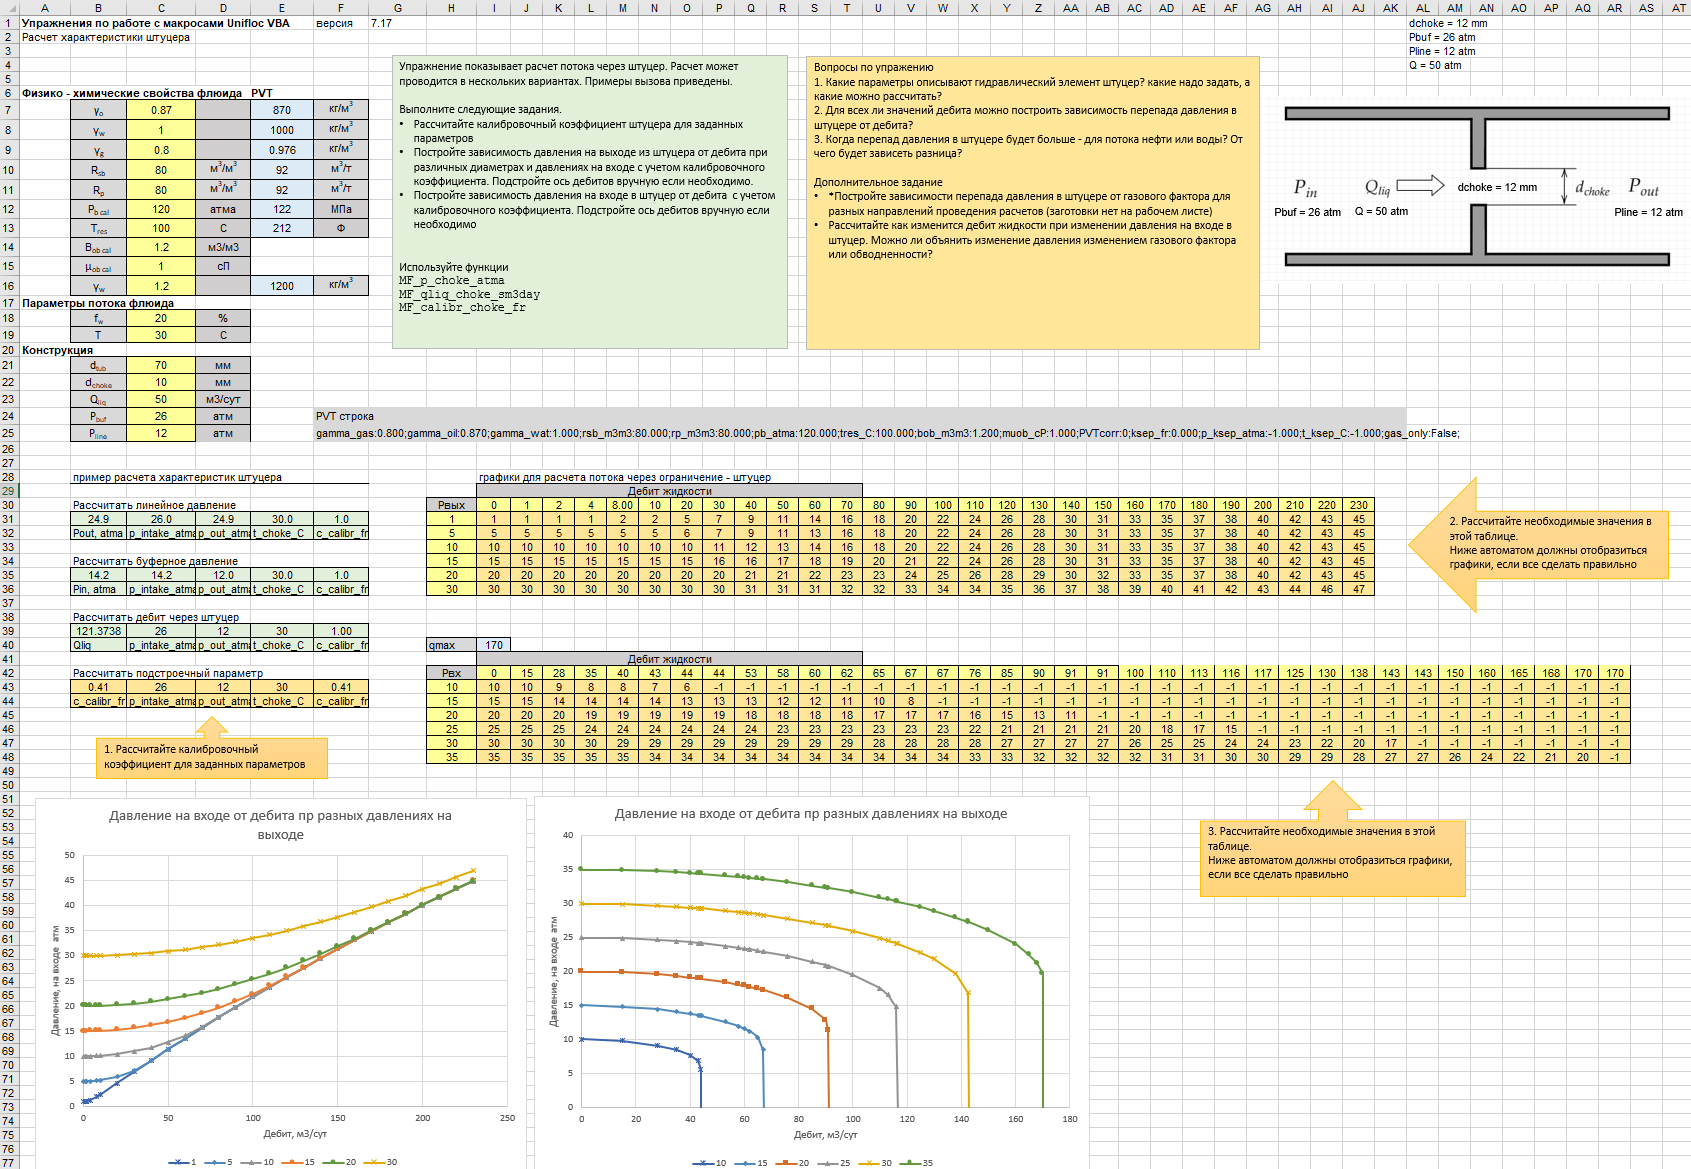
\includegraphics[width=1\linewidth]{Ex40_1}}
	\caption{Упражнение \mintinline{vb.net}{ex040.MF_choke.xlsx} со всеми заполненными полями }
	\label{ris:Ex40_1}
\end{figure}


\subsection{Упражнение}
Выполните следующие задания.
\begin{enumerate}
	\item Рассчитайте калибровочный коэффициент штуцера для заданных параметров
	\item Постройте зависимость давления на выходе из штуцера от дебита при различных диаметрах и давлениях на входе с учетом калибровочного коэффициента. Подстройте ось дебитов вручную если необходимо.
	\item Постройте зависимость давления на входе в штуцер от дебита  с учетом калибровочного коэффициента. Подстройте ось дебитов вручную если необходимо 
\end{enumerate}

Для выполнения расчетов используйте следующие функции \unf{}:
\begin{itemize}
	
	\item \mintinline{vb.net}{MF_p_choke_atma}
	\item \mintinline{vb.net}{MF_qliq_choke_sm3day}
	\item \mintinline{vb.net}{MF_calibr_choke_fr}
	
\end{itemize}

\subsection{Вопросы для самоконтроля}
Для самоконтроля ответьте на следующие вопросы:

\begin{enumerate}
	
	\item Какие параметры описывают гидравлический элемент штуцер? Какие надо задать, а какие можно рассчитать?
	\item Для всех ли значений дебита можно построить зависимость перепада давления в штуцере от дебита?
	\item Когда перепад давления в штуцере будет больше - для потока нефти или воды? От чего будет зависеть разница?
	\item Изменением каких параметров можно откалибровать расчет для штуцера? На что они влияют?
	
\end{enumerate}

\subsection{Дополнительные вопросы и задания}

Для того, чтобы глубже разобраться в расчете потока через штуцер с использованием \unf{} ответьте на дополнительные вопросы, которые легко превращаются в задания.

\begin{enumerate}
	
	\item  Постройте зависимости перепада давления в штуцере от газового фактора для разных направлений проведения расчетов. Чем зависимость будет отличаться от аналогичной для дебита жидкости? 
	\item Рассчитайте как изменится дебит жидкости при изменении давления на входе в штуцер. Можно ли объяснить изменение давления изменением газового фактора или обводненности?
	\item Рассчитайте работу штуцера для потока газа.  Как изменится перепад давления для газа по сравнению с ГЖС?
	
\end{enumerate}

Установите \mintinline{vb.net}{gas_only=True} для PVT строки для проведения расчета для газа. Расход газа при этом задается параметром \mintinline{vb.net}{q_gas_sm3day} в функциях расчета штуцера.